%!TEX root = ../thesis.tex

\cleardoublepage
\chapter{Evaluation}
\label{cha:evaluation}

This chapter reviews how the implementation from the previous chapter was tested, and discusses the observed results. This chapter will explain the setup of the testbed, as well as the motivation behind the types of tests which were performed. Finally a discussion of the results and their possible explanations will take place.


\section{Evaluating Performance}

\subsection{Testbed Setup}

In order to evaluate the success of the proposed approach a multipath scenario with four links will be emulated and investigated. Each test will consist of two WAN connectors and the four emulated links going between them. The characteristics of the links will be changed during the tests. For each test a different property will be investigated: latency, packet loss, and jitter. The evaluations will be performed on a testbed consisting of four seperate host servers. Two of these servers will run as the originating and terminating WAN Connectors. One server will generate and measure traffic. In between the two WAN Connectors, the final server will act as the link emulator. This architecture is shown in figure \ref{fig:testbed}

\begin{figure}[h]
    \centering
        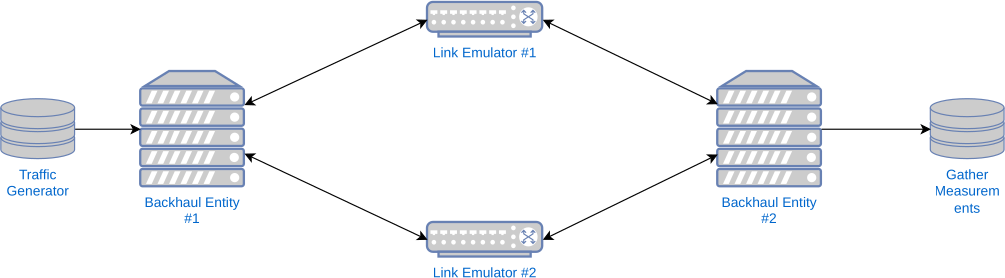
\includegraphics[width=0.66\textwidth]{fig/testbed.png}
        \caption{Testbed Setup}
        \label{fig:testbed}
\end{figure}

In figure \ref{fig:testbed}, the links between the servers are 1GB ethernet cables. The hosts are connected as is shown. In the “traffic generator and measurer" two linux namespaces are used to separate the traffic generation and the measurement. The packets generated in one namespace are routed via the ethernet connection to the next host (the terminating or “edge" WAN Connector). Because of the linux namespace the kernel is not aware that the packet's destination is technically the same host as itself. The packets are then are backhauled by the WAN Connector, over the emulated links in the next host and via the terminating WAN Connector, back to the original host, but now arrive in the “measurer" namespace.

The link emulation is done using the tc subsystem. First, a root Heirarchical Token Bucket (HTB) qdisc is established on the “downlink" and “uplink" interfaces of the link emulator. Secondly, the qdisc is given children classes, one class per emulated link. This allows one to establish bandwidth caps for each individual link being emulated. Within these HTB classes the root qdisc is a Network Emulator (NetEm) qdisc. The NetEm qdisc can be then configured to simulate characteristics such as latency, packet loss, and jitter.


In order to make the emulation more realistic, the NetEm qdiscs will be adjusted periodically. This allows one to degrade or improve links over time, for example by increasing the latency or packet loss in frequent intervals, until it reaches a large value. It also more closely mimics the real-life behavior of WAN connections, which do experience changes in their characteristics over time.

For the purposes of evaluating the WAN connector, three series of experiments will be performed to isolate and investigate it's link switching capabilities. First, purely latency based link selection will be investigated; a flow will be defined with specific latency requirements and then the emulated links will have their latency repeatedly changed. Then the same will be done once with packet loss and once with jitter. In each of these scenarios the other two parameters will be held constant, so that the WAN Connector can be judged based on its ability to meet one of the latency, jitter, or packet loss requirements, without the other two requirements interfering. In order to approximate realistic scenarios these experiments will also be repeated once with background traffic that aims to saturate the link's capabilities.

The data for the emulation used in all of these scenarios was obtained using the Satellite Constellation Network Emulator (SCNE) \footnote{https://connectivity.esa.int/projects/scne} from the European Space Agency. The default scenario is 24 hours long and consists of 288 satellites, 10 gateways (GW), and 50 user terminals (UT). The reason this data is used is twofold. Firstly, because LEO satellite links are likely to be the most common type of backhaul for geographically distributed 5G Campus Network deployments, and secondly, because LEO satellite connections are exceptionally more volatile than “regular" links \cite{deutschmann2022broadband} \cite{ma2023network}. By choosing to emulate more volatile links in the testbed, the WAN Connector experiences a more difficult test, and one can be assured that the real life performance in “normal" scenarios, is unlikely to be worse.

Since the WAN Connector is defined to work on at most four outgoing links, each investigated scenario will feature four links. These links will all be based on data from the SCNE emulation.

\subsection{Accuracy of the Emulation}

To make sure that the testbed emulation also matches the values from the SCNE, a brief comparison was done where the testbed's latencies were compared with those recorded in the SCNE. Since the SCNE runs over 24 hours but only records data every 10 seconds, the testbed's emulation was performed at a faster rate. The latency is adjusted each second instead. This helps to reduce the time needed to test the WAN Connector, and it makes the link appear even more volatile. This is once again not a bad thing, since it means the WAN Connector's performance can be seen as a lower bound. In realistic deployment scenarios the link's characteristics will be less volatile and the performance should be better.

Figure \ref{fig:sim_vs_em} shows the comparison between the data observed in the testbed, and the SCNE. The testbed data in the graphic is measured by the packet flows running over the individual links. The emulation data comes from the values recorded with the SCNE. Since the testbed data is collected at a rate of 100 packets per second, but runs at 10 times the speed of the SCNE emulation, there are 10 times as many data points. This explains why the graph of testbed data could be described as a blurrier version of the graph of the SCNE data.

\begin{figure}
  \centering
  \begin{tabular}{@{}c@{}}
    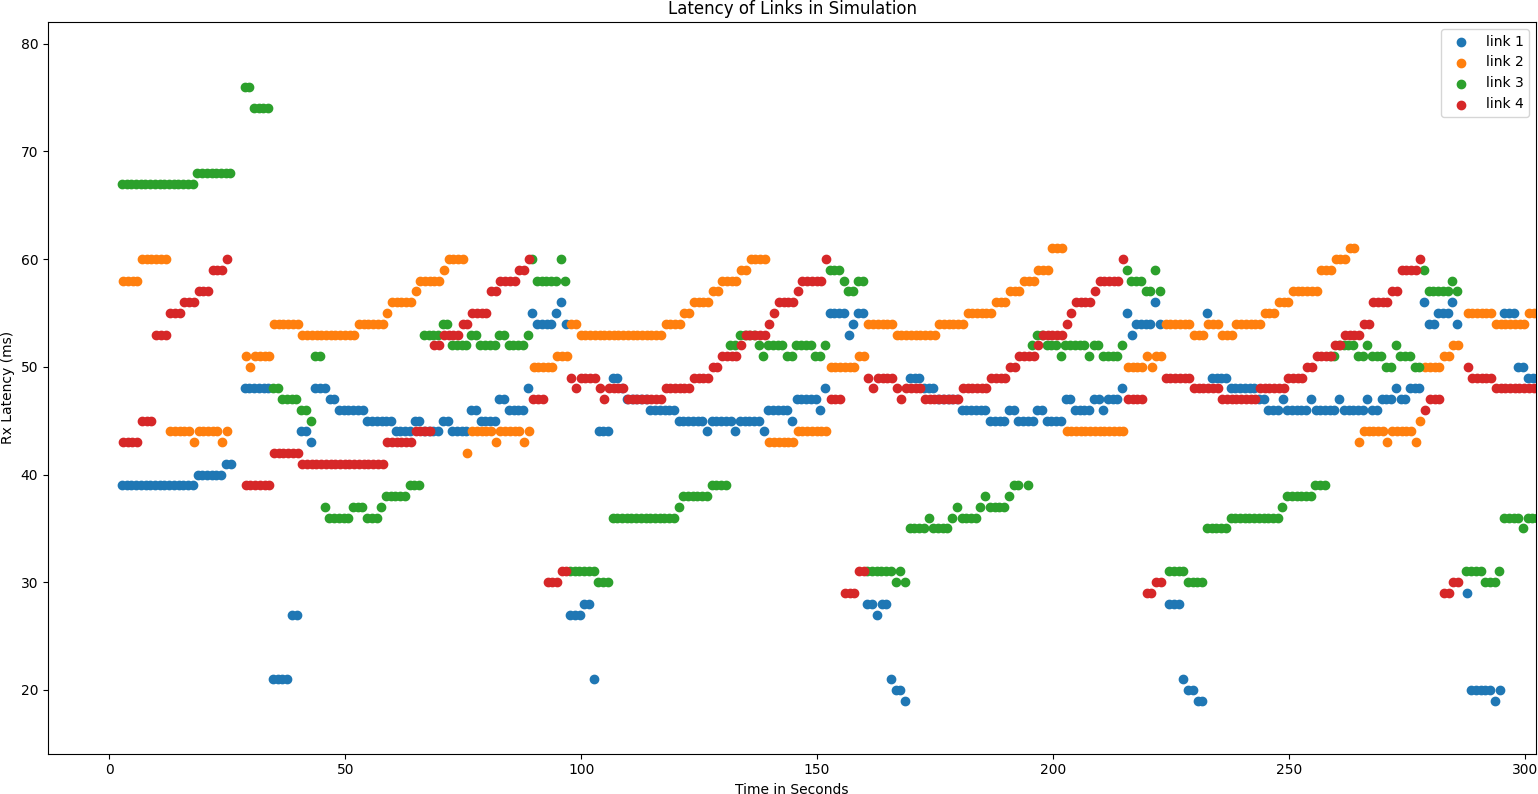
\includegraphics[width=\linewidth]{fig/simulated_latencies.png} \\[\abovecaptionskip]
    \small (a) Latencies Recorded in SCNE
  \end{tabular}

  \vspace{\floatsep}

  \begin{tabular}{@{}c@{}}
    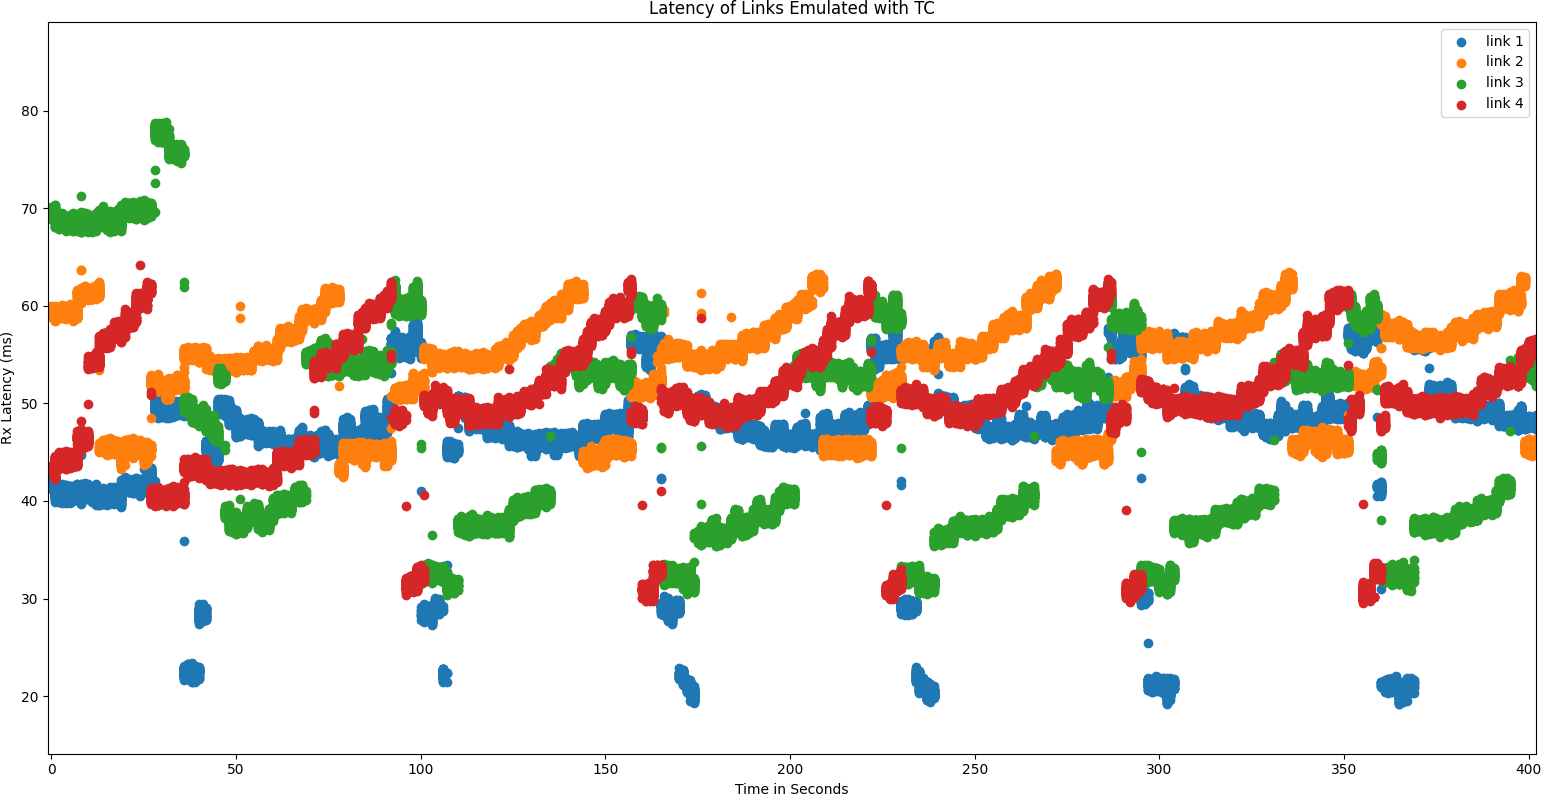
\includegraphics[width=\linewidth]{fig/emulated_latencies.png} \\[\abovecaptionskip]
    \small (b) Emulated Latencies Measured in the Testbed
  \end{tabular}

  \caption{Comparison of the Emulator's and the Testbed's Latencies}\label{fig:sim_vs_em}
\end{figure}

As can be seen in the figure, the latencies recorded on the testbed closely match those from the SCNE, which it was seeking to replicate.

\section{Latency Based Path Switching}

The first aspect with respect to which the WAN Connector is investigated is it's ability to provide a bound on latency. During the experiments the SCNE data is used to adjust the tc NetEm qdisc on the “link emulator" machine periodically. As was mentioned before, because the SCNE simulator provides latency data over a 24 hour period in 10 second intervals, the simulation data is “sped up". This means that the 24 hours of data can be cycled over in just 2 hours.

\subsection{Performance Compared to Single Links}

In this experiment both the WAN Connector and the links themselves are measured. This is done to have a comparison between the performance of the WAN Connector and the baseline performance level, which is the best performing link. The minimum acceptable performance of any path switching application is to provide a better performance than the best single link. Otherwise it would be better to just select the best link, and not use the application, or the other links, at all.

To give an idea of the best possible performance, the Oracle results are computed after the experiment.  The Oracle results are purely theoretical. For each packet, it is able to select the best path to forward on, based on that path's future characteristics. This approach is calculated by comparing the latency of each packet sent by the WAN Connector with the latency that that packet would have experienced on any of the other links. If the latency of the link chosen by the WAN Connector would be greater than the maximum acceptable delay for that flow, then the Oracle selects a different link with an acceptable latency (if one exists). Since it always picks an optimal path, the Oracle approach provides a hard upper bound on the best possible performance, and thus acts as a valuable comparison. It is important to note that the Oracle does not pick the path with the minimum latency, rather, it sticks with the WAN Connector's decision whenever that decision guarantees the latency bound, or there is no such decision is possible. Only if the WAN Connector's decision is wrong (the current path would give a latency that exceeds the bound, and there exists a different path which would provide latency below the bound), does the Oracle select a different path.

In the experiment a flow is defined in the WAN Connector with a minimum round trip time (RTT) of 56 milliseconds. This value is chosen because it is the mean of the means of the latencies of the four links in the emulation. For the evaluation of the latency based path switching, packets which match the flow definition are sent at a rate of 100 per second. In order to serve as a comparison, identical 100 packet per second flows are sent across the four other links. Along with the WAN Connector's latnecies, the latencies measured on the four links are used to calculate the Oracle approach's results.

The graphics \ref{fig:latency_cdf1} and \ref{fig:latency_cdf1_super_zoomed_in} show a cumulative distribution of the different latencies experienced by the packet flows running over the individual links and over the WAN Connector, as well as the theoretical performance of the Oracle approach.
\begin{figure}[h]
    \centering
        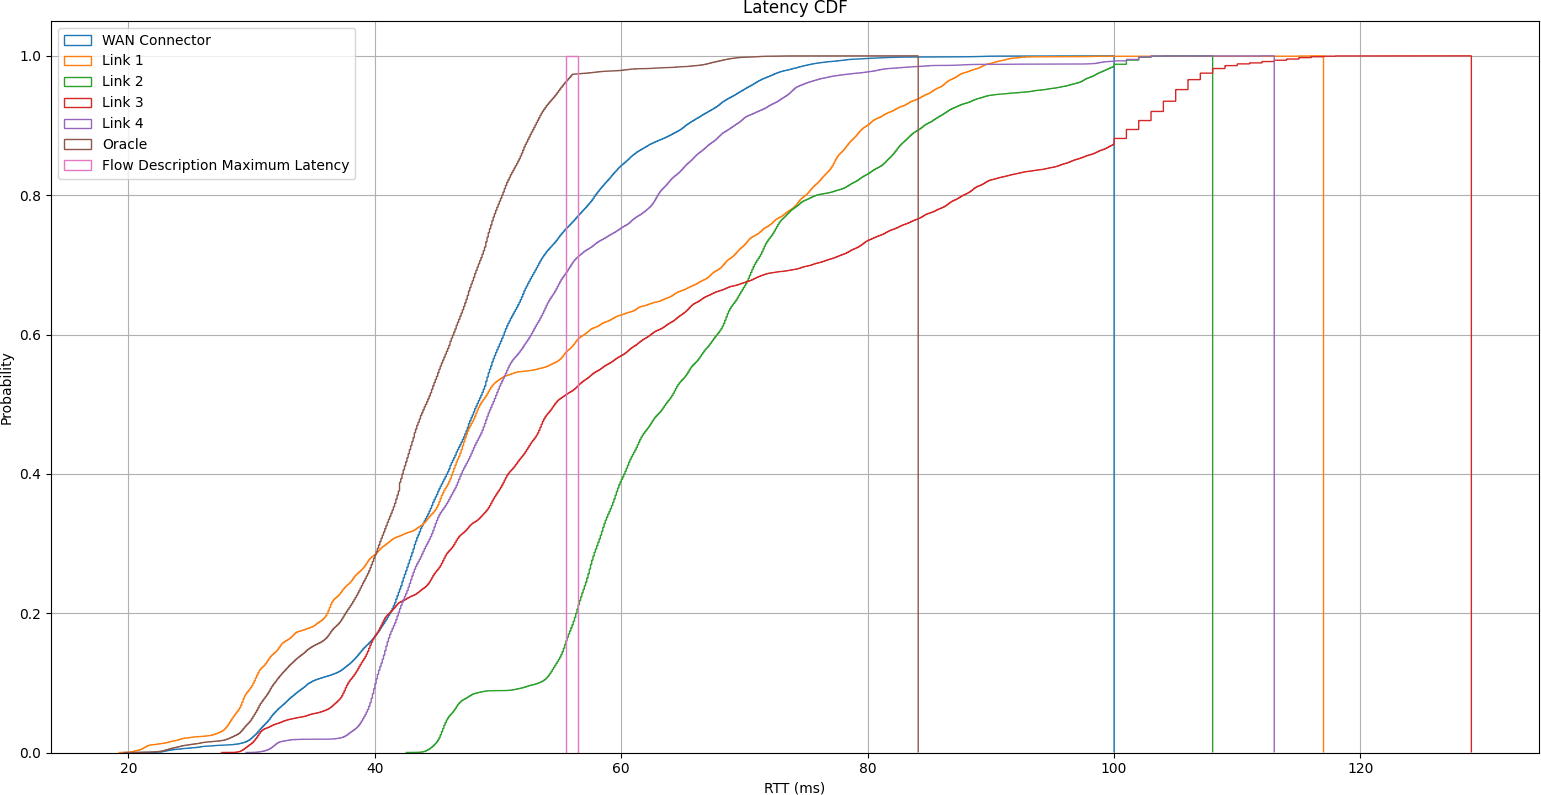
\includegraphics[height=0.8\textwidth,width=\textwidth]{fig/latency_cdf1.png}
        \caption{Cumulative Distribution of the Latencies}
        \label{fig:latency_cdf1}
\end{figure}

\begin{figure}[h]
    \centering
        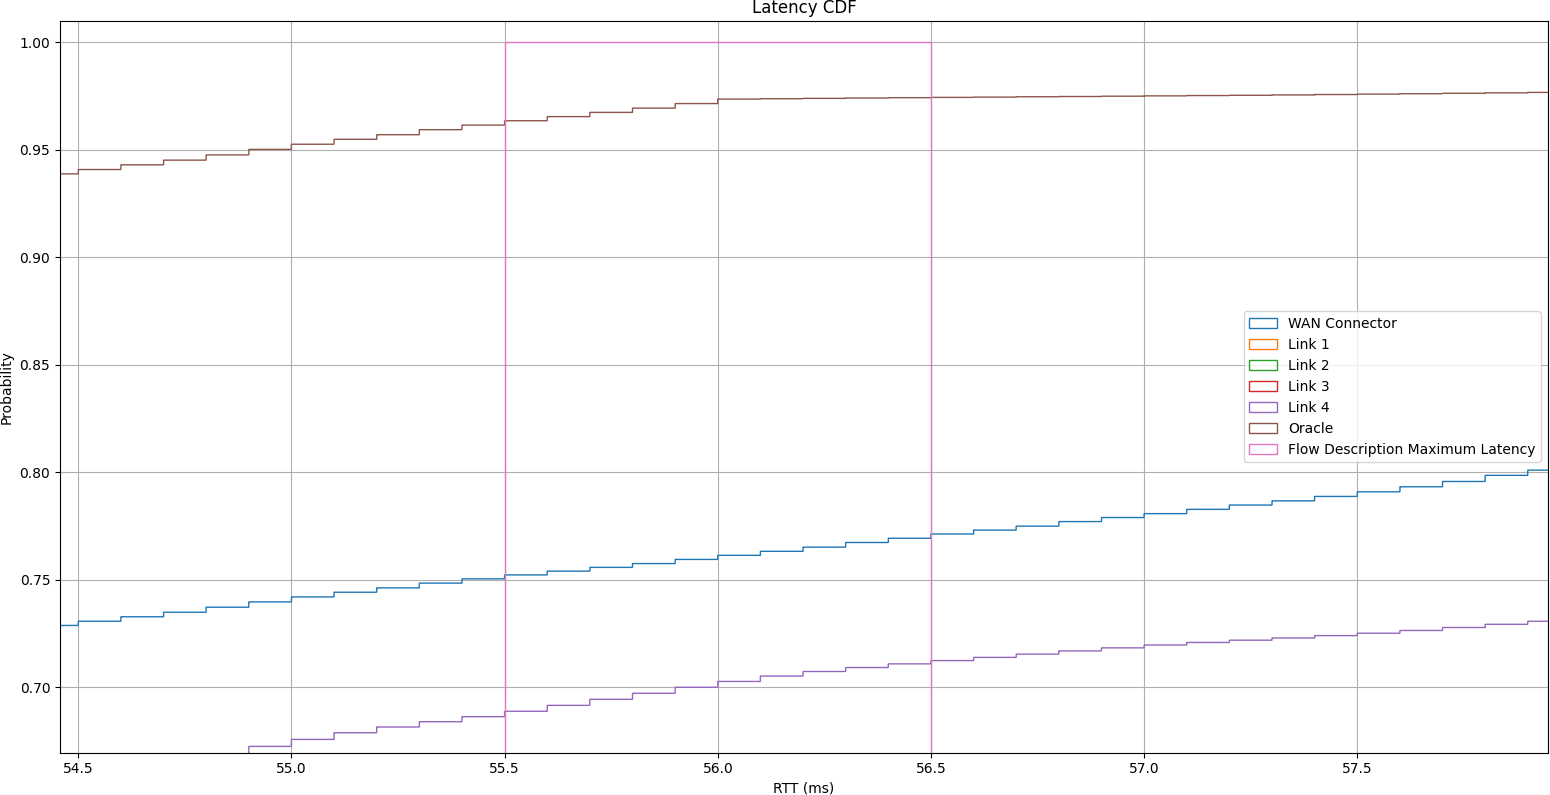
\includegraphics[height=0.66\textwidth,width=\textwidth]{fig/latency_cdf1_super_zoomed_in.png}
        \caption{Closeup of the Latency CDF}
        \label{fig:latency_cdf1_super_zoomed_in}
\end{figure}

The CDF shown in figure \ref{fig:latency_cdf1} and zoomed in on in figure \ref{fig:latency_cdf1_super_zoomed_in} tracks the probability that the flow experiences a latency less than or equal to the latency value on the y axis. The pink bar labeled “Flow Description Maximum Latency" is set at 56 milliseconds and represents the latency bound for the flow being measured. The ideal performance would have the entire CDF end within or before the pink bar, as that would mean that no packet for the flow experienced a latency greater than 56 milliseconds.


The results in the figures show that the WAN Connector is able to achieve a superior performance to any of the individual links on their own. This was the baseline requirement and it is important that it is able to achieve this. However the performance does not significantly improve on the next best link, which is able to provide latency below the maximum allowed latency 72\% of the time, while the WAN Connector does so 77.5\% of the time. The Oracle approach shows that in theory one could, at best, have maintained the flow's latency bound 97.5\% of the time. This means the WAN Connector's performance is 80\% optimal.


\subsection{Latency Performance Under Load and the Importance of Traffic Shaping}

During this experiment, the same 100 packet per second flow from before is repeated, but background traffic is added. An iperf3 \footnote{https://iperf.fr/} test is run across the WAN Connector at the same time as the latency critical flow, and the background traffic is given the same latency requirements, so that the WAN Connector always schedules both flows to the same link. This ensures that whatever link is being used will be saturated. Latency performance during congestion is a crucial element of a deterministic backhaul solution. The WAN Connector's control plane only makes the decision about which link to forward on- it does not perform load balancing or prioritization. The data plane does not do this either, it implements a purely First In First Out (FIFO) approach to packet queuing. This decision was made because the burden of implementing an appropriate packet shaper, in addition to the other multipath calculations, is too significant for the purposes of this thesis, and because powerful traffic shaping implementations which can be integrated into this solution already exist.

\begin{figure}[h]
    \centering
        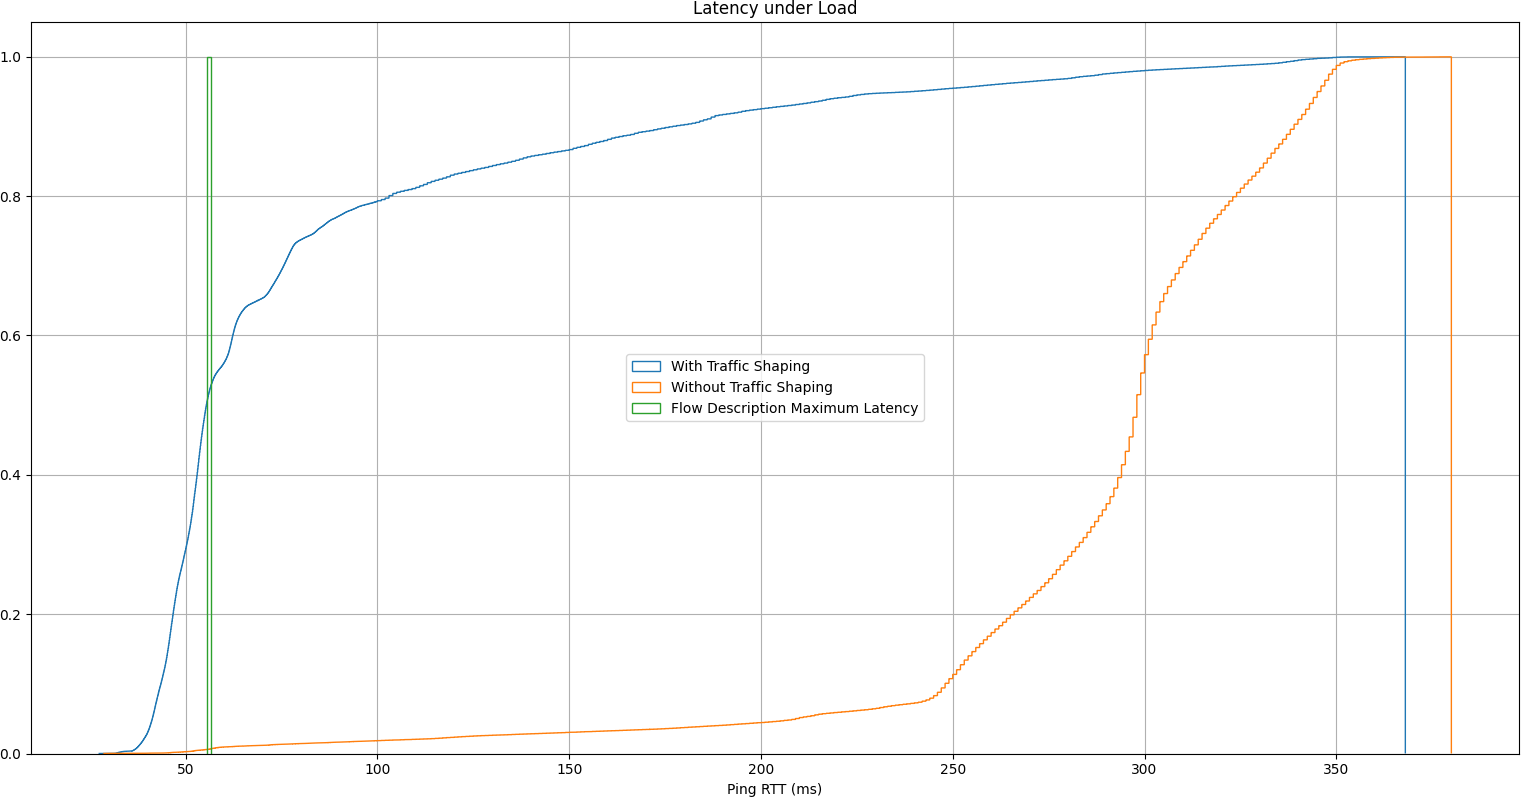
\includegraphics[height=0.66\textwidth,width=\textwidth]{fig/rrul_cdf.png}
        \caption{Latency with Background Traffic}
        \label{fig:rrul_cdf}
\end{figure}

Figure \ref{fig:rrul_cdf} neatly demonstrates why traffic shaping is an essential element of any deterministic network. In the case in which there is no traffic shaper the latency critical flow experiences significant additional latency due to the network being overloaded. The TCP algorithm fills the link's capacity, and the latency critical packets spend too much time buffering and arrive late. It should be noted that the WAN Connector's performance under load is worse than in the previous test, where there was no background traffic. 50\% of the packets experience latencies less than the maximum allowed delay which was defined for the critical flow. However the approach without the traffic shaping fares much worse and can only provide an acceptable delay 1\% of the time.

\section{Reliability Based Path Switching}

In the next scenario, to analyze the ability of the WAN Connector to achieve the required reliability of a given flow, the same test flows from before are run over the WAN Connector and the four outgoing links. However this time instead of varying the latency, the packet loss ratio of the link is changed. The SCNE emulation's data is used for the testbed once again. However since the emulation does not provide packet loss statistics on a per second basis, the latencies of all the different links in the simulation are used. For the emulation, these 51 values are looped over in 10 second increments. Each link is given a shuffled set of these 51 values. This means that the cumulative value of the packet loss experienced by all of the links is the same (2\%), but the instantaneous values will differ. To appropriately analyze this scenario the flow being backhauled over the WAN Connector is given a reliability threshold of 0.1\%. This is because in this scenario, where the existing links all provide an average of 2\% reliability, setting a lower threshold means that it becomes necessary to duplicate packets at some points, in order to achieve the required reliability. Afterwards, the experiment is repeated under load, just like during the latency investigations. For the reliability under load scenario a second iperf3 flow is run across the WAN Connector in order to saturate the link. Like before, this second flow is given the exact same requirements as the test flow, to ensure that they are always scheduled across the same link by the path selection algorithm.

Just like before, the results achievable by an Oracle are calculated.  This time the Oracle approach is defined as choosing, before forwarding any packet, the link with the lowest packet loss ratio. But, crucially, the Oracle is not allowed to duplicate flows across different links. The Oracle is not able to predict the loss of individual packets, it only knows the overall probability that a packet will be lost if it is sent on a given link, and it always selects the link with the lowest probability.

\subsection{Packet Loss Measurements}

 The results of this experiment are shown in figure \ref{fig:loss_bars1}. The packet loss recorded by each of the flows over the entire experiment is plotted in a bar graph, as well as the theoretical packet loss which would have been experienced by the Oracle approach. For the sake of the reader, another bar is plotted which represents the target reliability that was requested by the critical flow.

\begin{figure}[h]
    \centering
        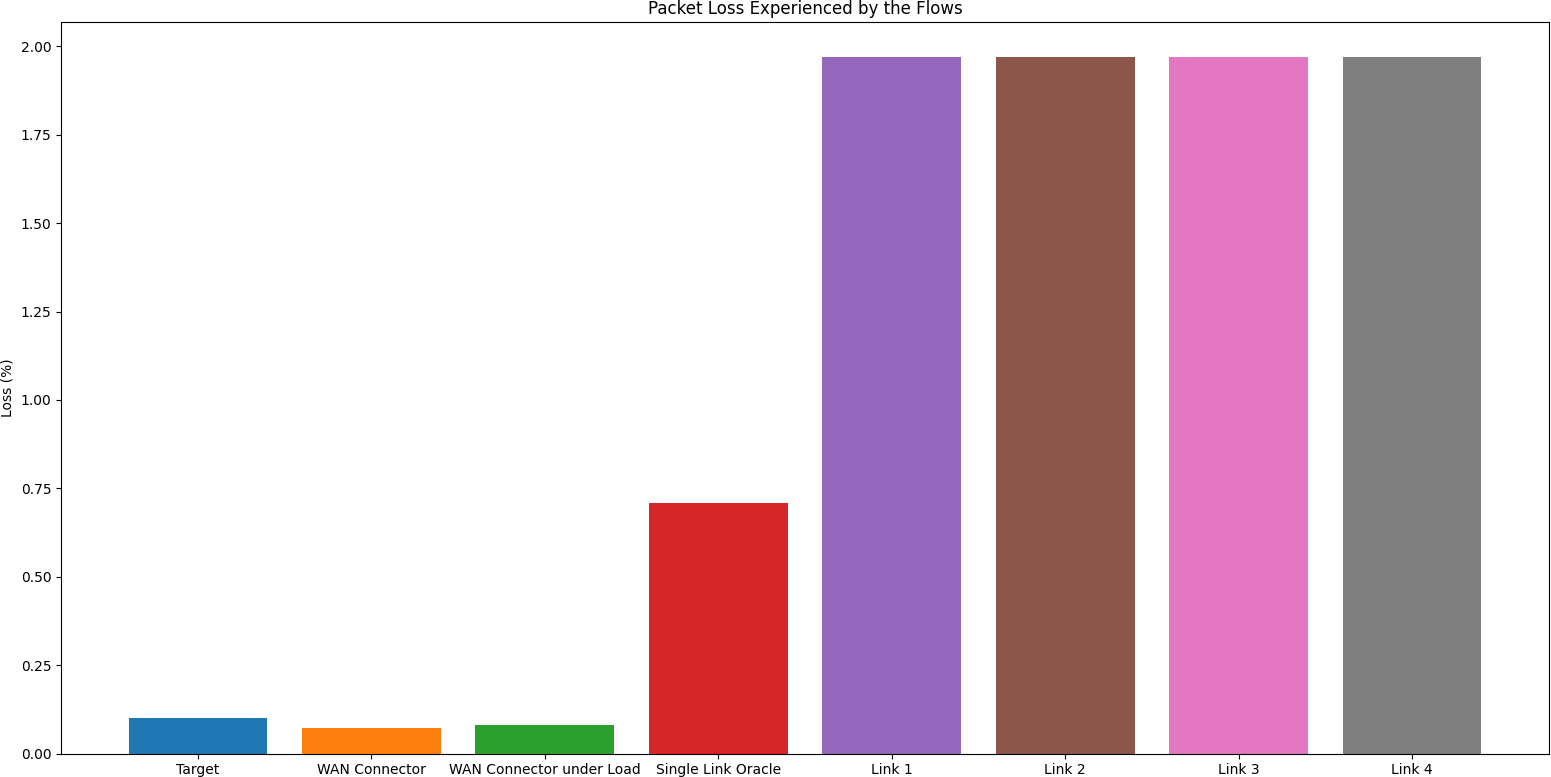
\includegraphics[height=0.66\textwidth,width=\textwidth]{fig/loss_bars1.png}
        \caption{Reliability}
        \label{fig:loss_bars1}
\end{figure}

As can be seen in figure \ref{fig:loss_bars1} all of the links, including the Oracle, are outperformed by the WAN Connector. The fact that the WAN Connector does better than the Oracle is because the Oracle is not allowed to perform frame replication. Indeed, as the graphic shows, it is not possible to achieve the critical flow's required reliability with any of the available links, nor with the Oracle approach, but the WAN Connector is able to achieve it. This speaks to the potency of the flow duplication approach, which is made possible in the optimization equation used to decided on which flows to forward.

\subsection{Caveat: Impact on Throughput}


\begin{figure}[h]
    \centering
        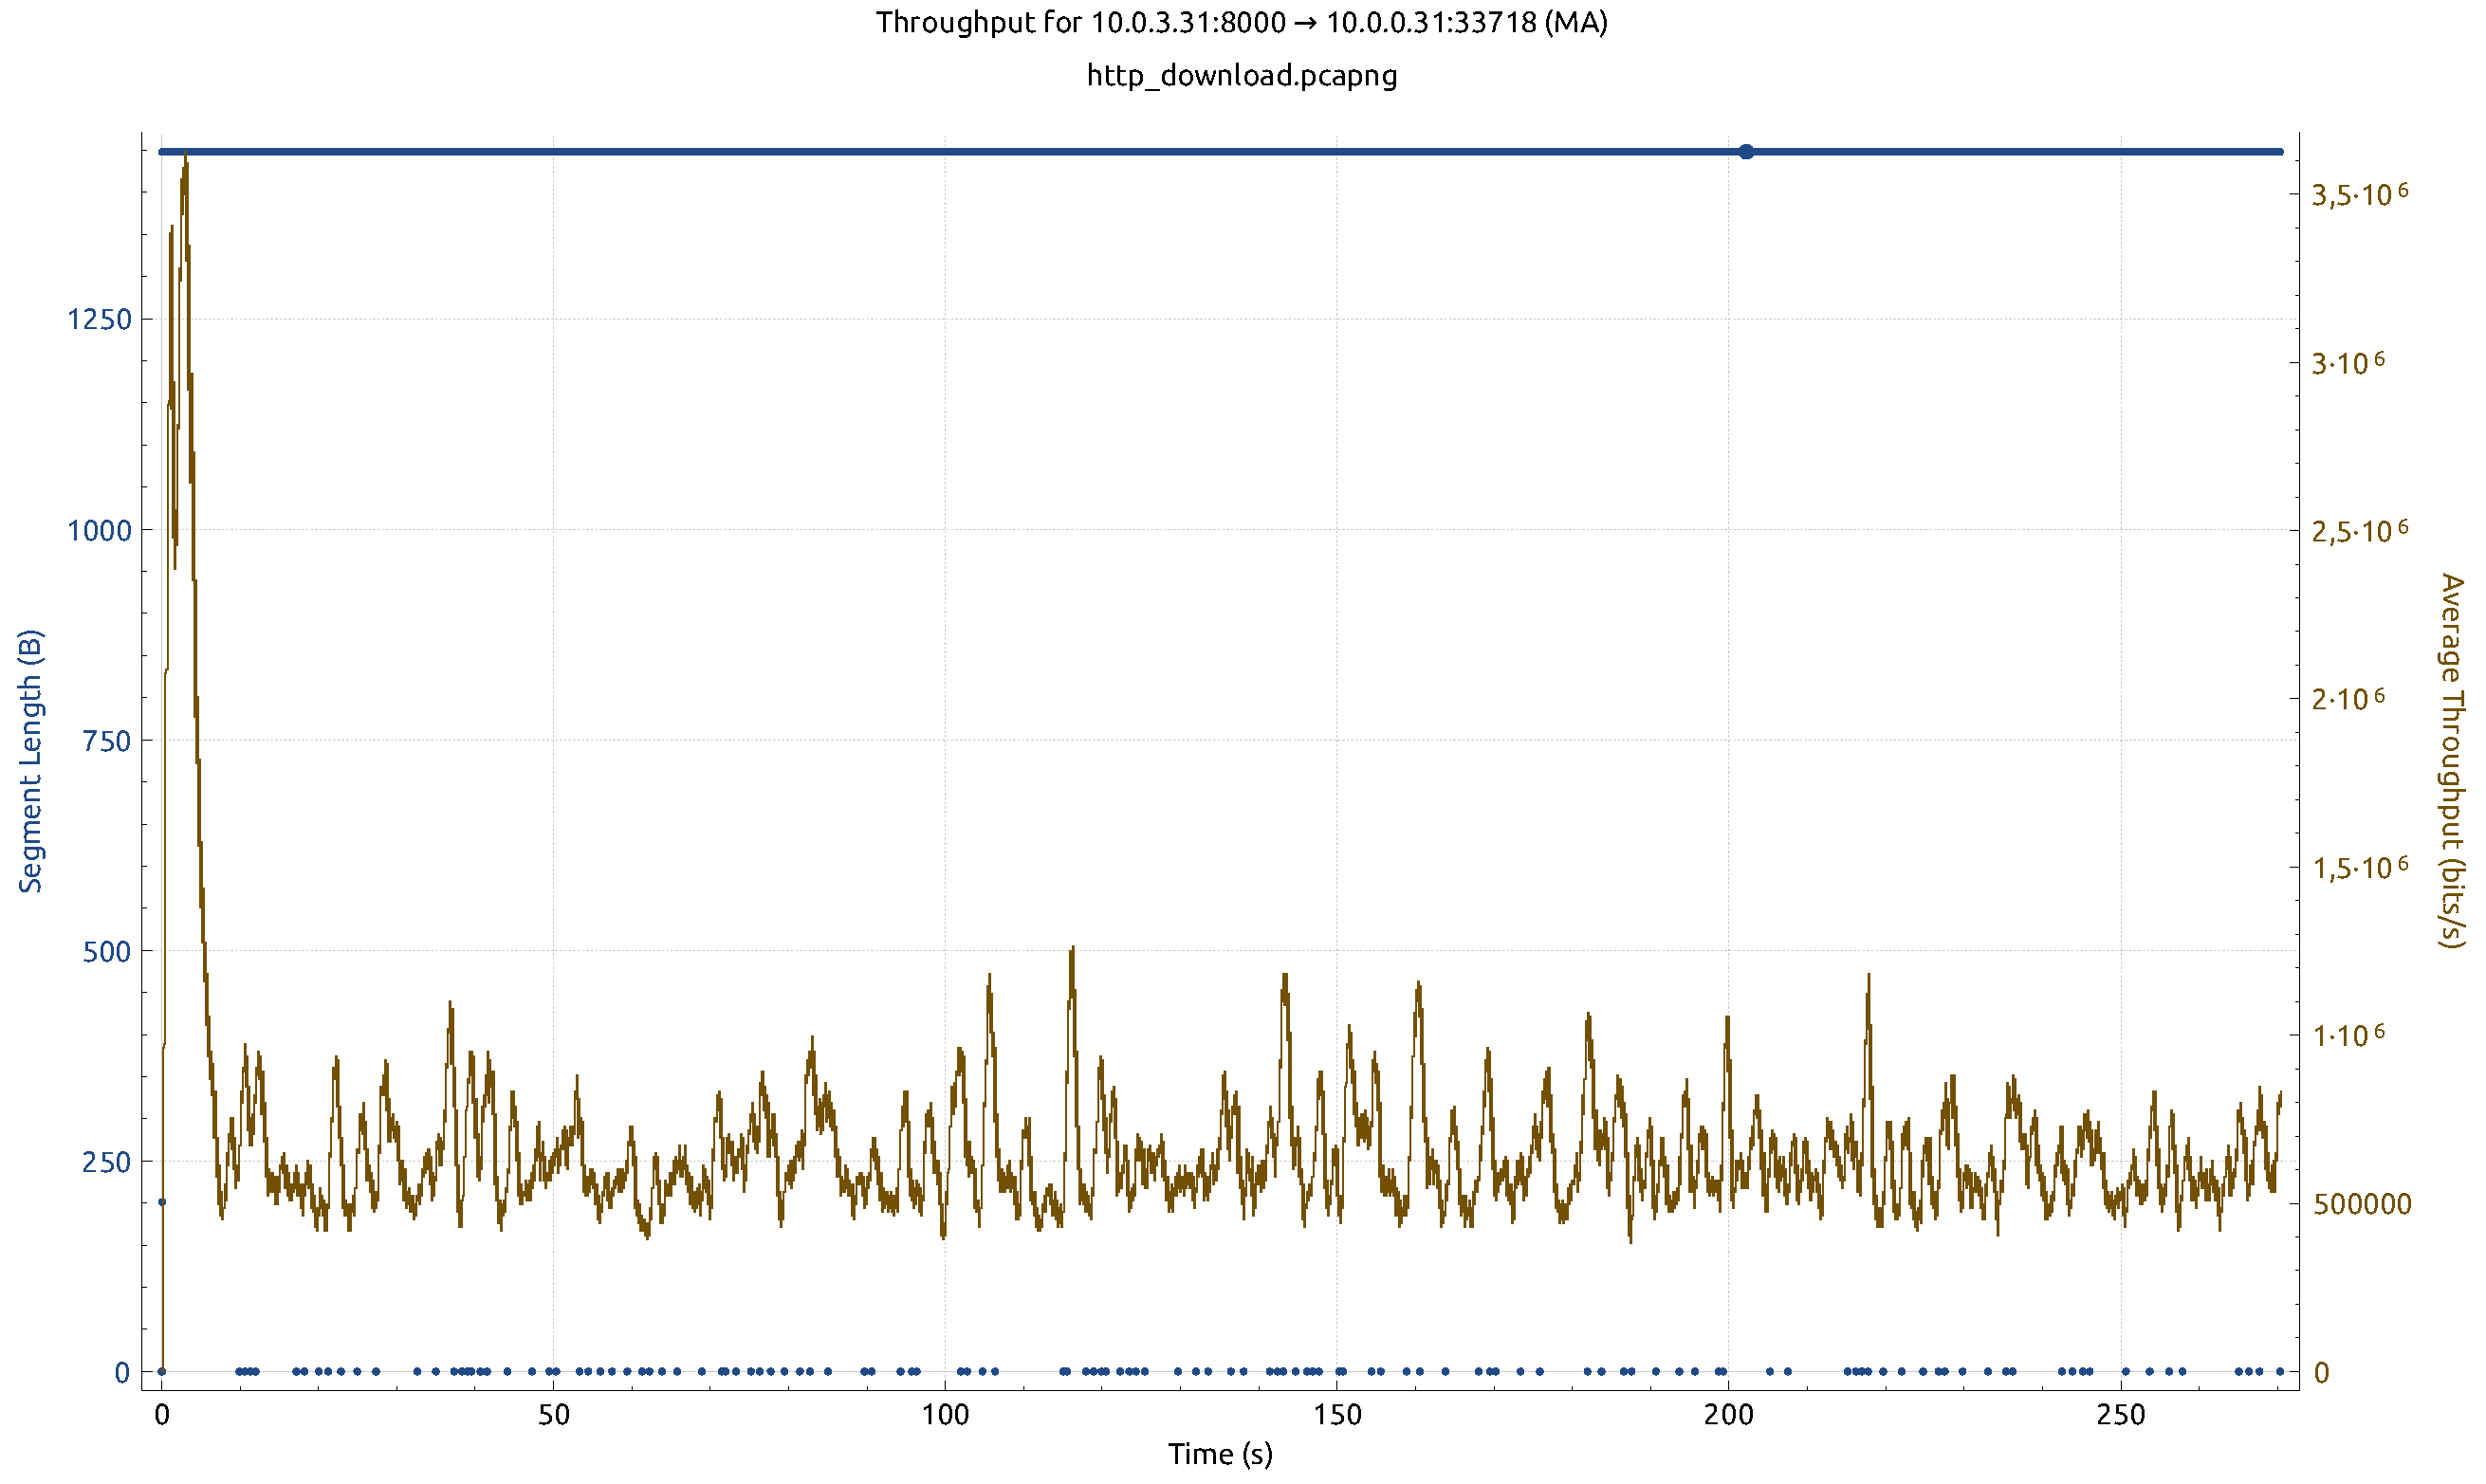
\includegraphics[height=0.66\textwidth,width=\textwidth]{fig/tcp_throughput.pdf}
        \caption{Throughput of a Duplicated Flow}
        \label{fig:dup_tcp}
\end{figure}

One of the unfortunate impacts of packet duplication is that it reduces the available bandwidth. In the worst case, where every flow must be duplicated, it represents a waste of 50\% of the total resources available. Additionally, since flows which are being duplicated need to be re-ordered, this means that the FIFO approach for packet queuing cannot be used, and instead the packets must pass through a Packet Ordering and Elimination Function (POEF). When a packet arrives out of order the POEF starts to incur significant additional overhead because it must store all packets until the missing packet arrives, or a point is reached at which the stored packets must be dequeued. This point is either the point at which the packets expire, or the queue of out of order packets becomes full. Beyond this, the storing and eventual mass de-queuing of out of order packets can also interfere with the TCP algorithm- thus leading to reduced throughput.

These two effects- the POEF overhead and the occasional appearance of duplicate packets- lead to a heavily reduced throughput, as can be seen in figure \ref{fig:dup_tcp}. The graph in the figure was generated by wireshark \footnote{https://www.wireshark.org/} based on the packet trace of a file download. It shows the segment-length and throughput experienced by the TCP stream running over the WAN Connector and experiencing replication. As can be seen in the graph, the throughput is low, and is not able to saturate the link's bandwidth despite being the only flow running at the time.

\section{Jitter Based Path Switching}

\begin{figure}[h]
    \centering
        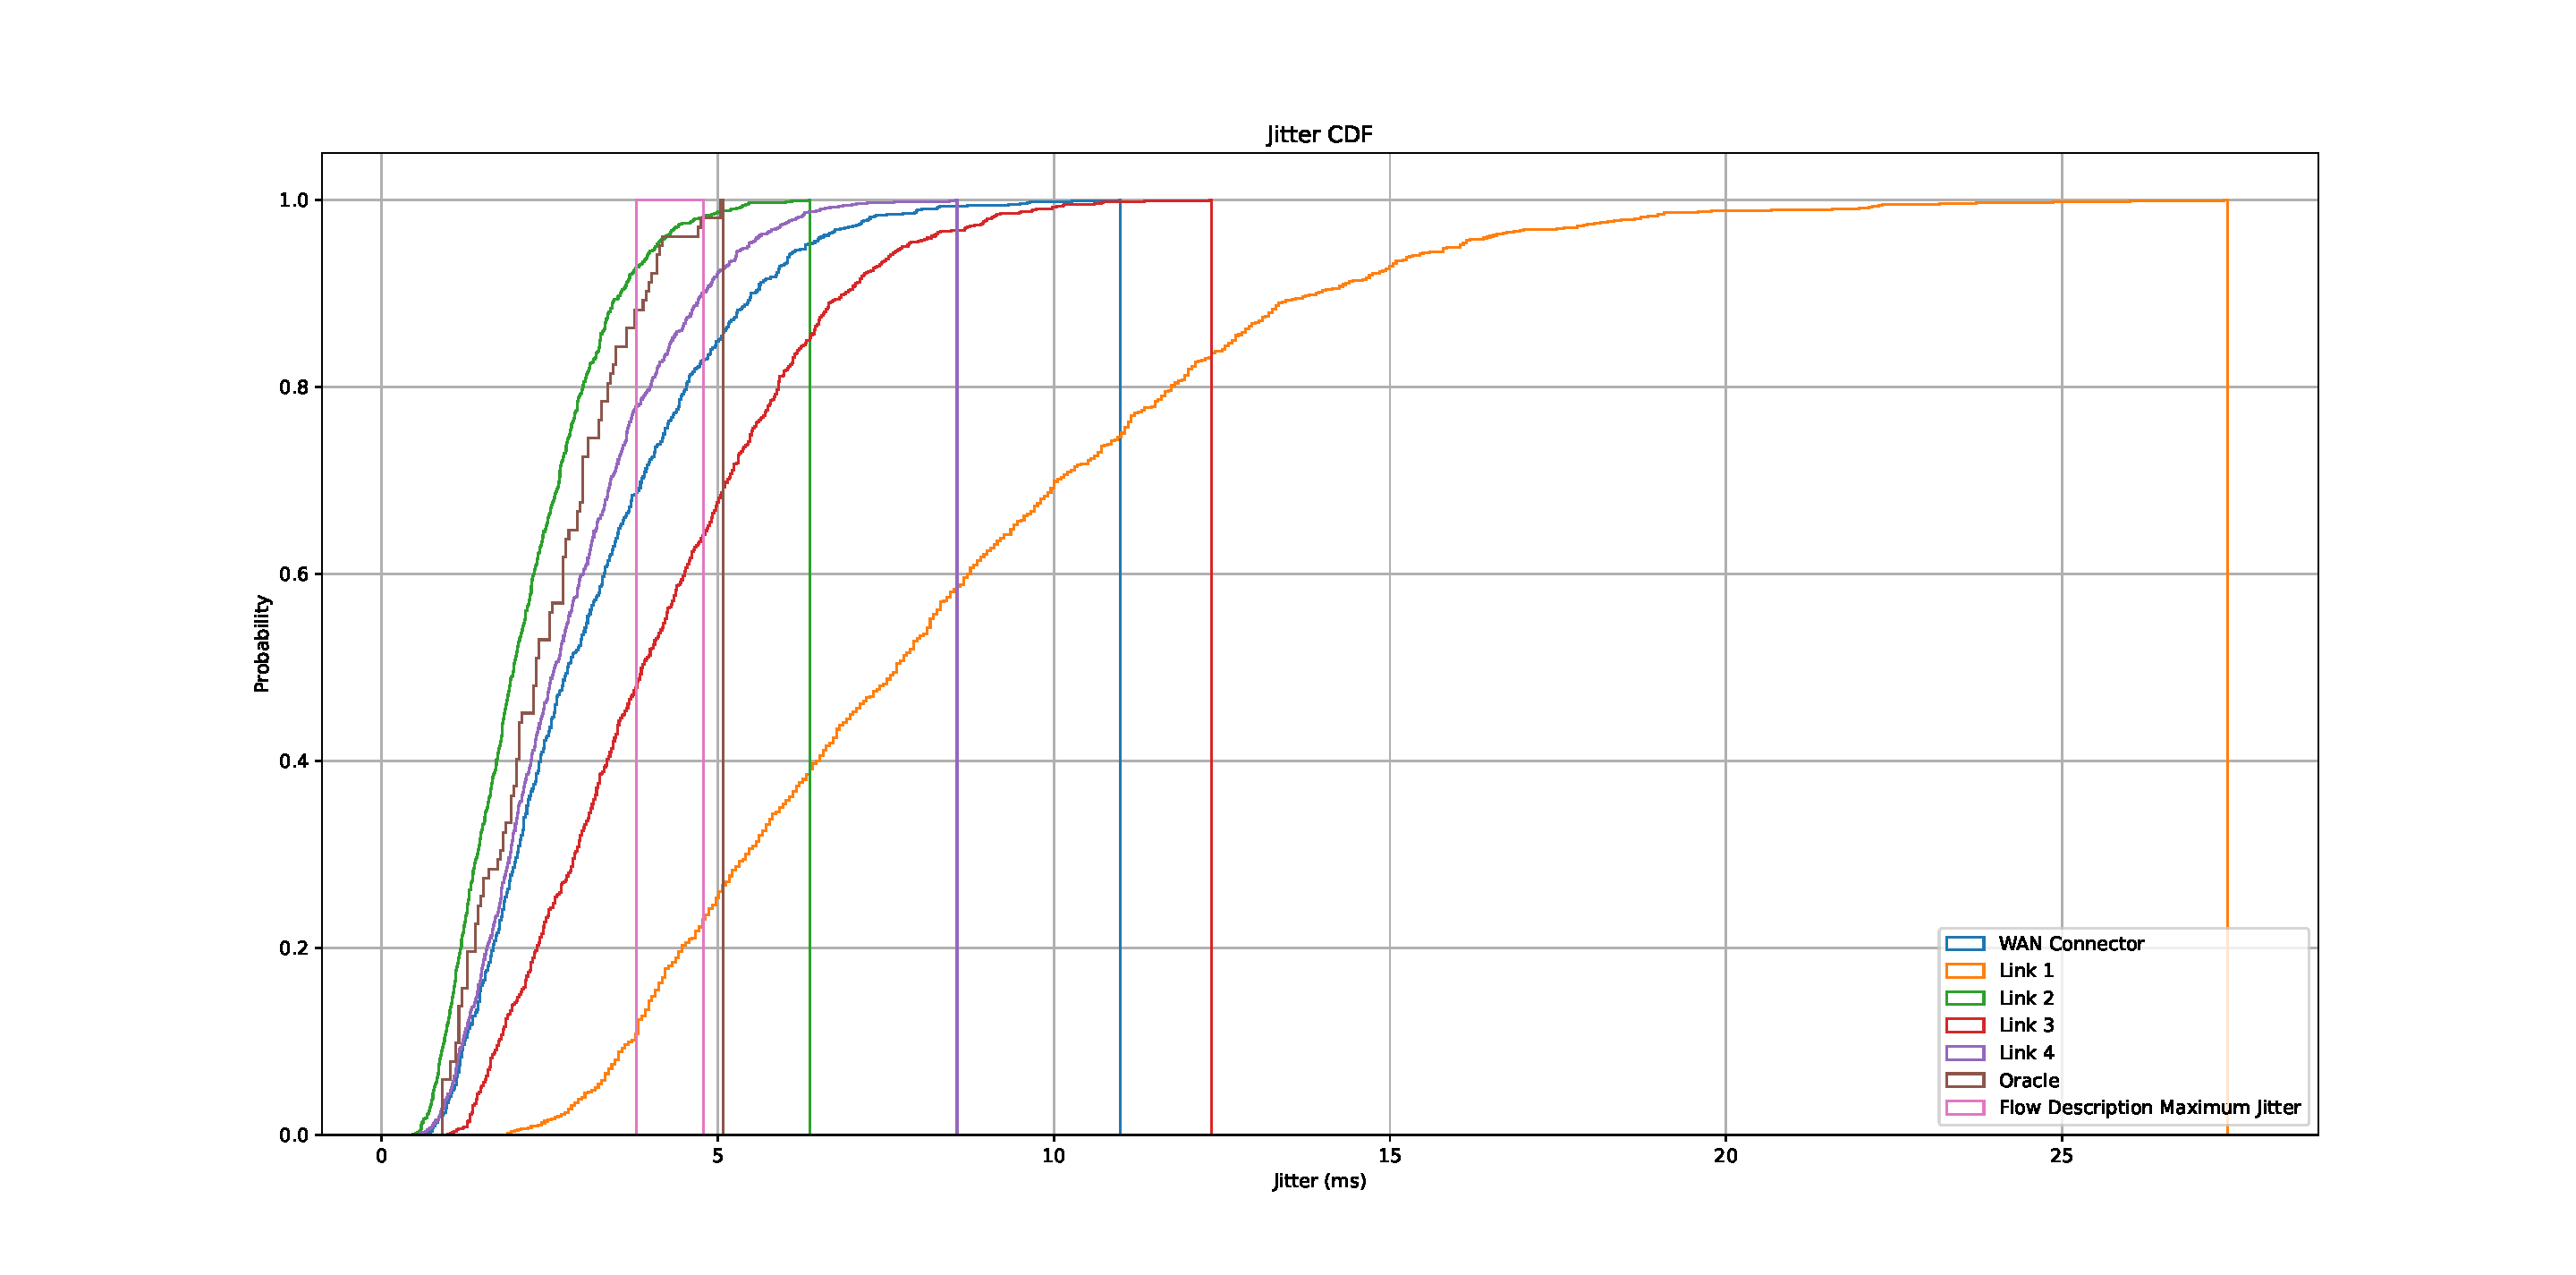
\includegraphics[height=0.66\textwidth,width=\textwidth]{fig/jitter_cdf.pdf}
        \caption{Performance of Jitter Based Path Switching}
        \label{fig:jitter_cdf}
\end{figure}

For the final analysis, the jitter must be investigated. For this purpose the simulation data was once again adapted. This time the standard deviation of the latency experienced was calculated for each of the 102 connections in the simulation. Then these standard deviations were scaled down by diving them by one, two, three, and four, respectively, in order to acquire four different set of jitter characteristics. Finally the scaled values were shuffled. This resulted in 4 links with varying jitter characteristics, which suffices for the emulation. Each different jitter value is emulated for 10 seconds on the respective link. During the emulation scenario a UDP iperf3 stream is ran at a rate of 3/4ths of the link's maximum bandwidth for 1000 seconds. The iperf3 tool records jitter each second, and this data is used to then analyze the performance.

Since more than half of the link capacity is being used by the flows being sent on the links, the WAN Connector cannot be tested at the same time. Thus, to test the WAN Connector the emulation is repeated but with the flow only being sent over the WAN Connector. Lastly, the Oracle approach is calculated based on the simulation data. The Oracle approach, like before, displays the theoretical optimal performance. It chooses, at each point in time, the link with the lowest jitter. The cumulative distribution of the jitter experienced by the flows is plotted in figure \ref{fig:jitter_cdf}.

As can be seen from the figure, the WAN Connector's performance is disappointing. It displays an inferior performance to two of the links. This means the path switching is actually causing a worse performance. This is most likely down to insufficient statistics causing poor path selection, because jitter statistics can't be gathered about other paths in this single flow scenario. The probe packets which are periodically sent out do not provide enough data points to accurately determine jitter. While they can give a sufficient baseline for latency calculations, as well as helping to determine if a link is dead or alive, their jitter measurements are not likely to provide a strong insight into the true nature of the link's jitter.

A final note about the plot in figure \ref{fig:jitter_cdf}. In the figure, link 2 actually performs better than the Oracle for most jitter values, before ultimately proving to have the greater maximum values. This occurs because the Oracle is based on the simulation data and not the measurements. Therefore there are more data points available for the link than for the Oracle, and the percentage of packets below a certain level of jitter is thus greater. However ultimately the maximum values experienced by the flow, during those times when the link experiences it's worst jitter, are worse than the Oracle approach's worst cases, and, as one would expect, the Oracle's CDF terminates before link 2.


\section{Assessment}

In light of these results one can conclude that the approach presented in the previous chapter is not without its flaws, however the results have also highlighted some of the functional aspects that were important for good performance. For latency based path switching it was able to outperform the other available links and achieve 80\% optimality, and the inclusion of a traffic shaper proved vital for preventing the latency critical flow from experiencing higher buffering times in the presence of a competing flow.

With regards to reliability, the WAN Connector showed that it was able to guarantee a critical flow a lower level of packet loss than would have been possible using any single link. Furthermore, it was even able to outperform the single link Oracle. In a situation where the single link Oracle was unable to provide the required minimum level of packet loss for the desired flow, the WAN Connector was able to deliver the desired reliability. This is a hugely important result because it shows that the WAN Connector can provide greater reliability, via packet replication, than even an optimal single link path selection algorithm. This can enable critical applications to run in environments where the backhaul options would usually be too unreliable to enable the critical applications.

This chapter, however, also demonstrates the downside of the packet replication approach, as it greatly reduces the overall throughput. Beyond this, during the jitter experiments, it is seen that the WAN Connector provides a poorer performance than simply using a single link for the entire experiment. This is fundamentally a bad result. The baseline by which any path selection algorithm should be judged is its ability to outperform the individual paths, since in theory it could always select a superior option when one exists. Since the WAN Connector fails in this instance it must be concluded that it cannot provide a reduction in jitter for those applications which are jitter sensitive. The author would suggest, however, that the problem in this respect is not due to the design but rather the implementation. Ultimately there was not enough accurate information about the jitter of the available links so that the path selection algorithm could choose the right one.












